
 \clearpage
 %%%%%%%%%%%%%%%%%%%%%%%%%%%%%%%%%%%%%%%%%%%%%%%%%%%%%%%%%%%%%%%%%%%%%%%%%%%%%%%%%
 %%        %%%        %%%        %%%        %%%        %%%         %%%  %%%%  %%%
 %%  %%%%%%%%%  %%%%%%%%%  %%%%%%%%%%%%  %%%%%%%%%  %%%%%%  %%%%%  %%%    %%  %%%
 %%        %%%        %%%  %%%%%%%%%%%%  %%%%%%%%%  %%%%%%  %%%%%  %%%  %  %  %%%
 %%%%%%%%  %%%  %%%%%%%%%  %%%%%%%%%%%%  %%%%%%%%%  %%%%%%  %%%%%  %%%  %%    %%%
 %%        %%%        %%%        %%%%%%  %%%%%%        %%%         %%%  %%%   %%%
 %%%%%%%%%%%%%%%%%%%%%%%%%%%%%%%%%%%%%%%%%%%%%%%%%%%%%%%%%%%%%%%%%%%%%%%%%%%%%%%%%
 \section{treeに出会う}

 \ROOT には拡張子に\verb|.root|を拡張子としたファイルがある。
 (以下\verb|root|ファイルと呼ぶ。)
 ここでは\verb|root|ファイルにデータを詰める方法とその使い方を示す。
 やることは
 \begin{enumerate}
  \item startとstopの2行が書かれたデータを開く
  \item startとstop、及びその差を読んでTDCの値とする。
  \item start、stop、TDCの値をTreeというものに格納する。\\
	\url{http://root.cern.ch/drupal/content/ttree-and-its-data}
  \item Treeを\verb|root|ファイルに書き出す。
 \end{enumerate}

 \begin{itembox}{\texttt{meettree.cpp}}
\begin{verbatim}
	#include <fstream>
	#include "TFile.h"
	#include "TTree.h"

	TTree *meettree(char *datafile, char *rootfile = "output.root"){

	double start ; // TDC start
	double stop  ; // TDC stop
	double tdc   ; // delta T

	TTree *tree = new TTree("tree","tree");  //TTree作成
	//Branch準備
	tree->Branch( "start", &start, "start/D" ); // start を格納する為のブランチ
	tree->Branch( "stop" , &stop , "stop/D" );  // stop を格納する為のブランチ
	tree->Branch( "tdc"  , &tdc  , "tdc/D" );   // start とstopの時間差 を格納する為のブランチ

	ifstream fin(datafile) ;
	while(fin >> start >> stop){
	tdc = stop - start ;
	tree->Fill() ;
	}

	TFile *fout = new TFile(rootfile, "recreate");
	tree->Write(); // treeを書き込む
	fout->Close(); // file close

	return tree ;
	}
\end{verbatim}
 \end{itembox}

  \subsection{\texttt{meettree.cpp}を実行する}
\begin{verbatim}
	$ root
	root [0] .L meettree.cpp+
	root [1] meettree("output.plt","test.root")
	(class TTree*)0x7fc1d22a1b70
\end{verbatim}
すると、作業ディレクトリに\verb|test.root|というファイルが出来ている。
(出力ファイルのデフォルト名は\verb|output.root|なので、\verb|meettree|実行時に第二引数を指定しなかった場合、
出来上がる\verb|root|ファイルは\verb|output.root|である。)
これが\verb|root|ファイルである。

  \subsection{Treeを扱う}
  以降、前節で出力したファイル名が\verb|test.root|だとして話を進める。
  \verb|test.root|に収められているTreeの扱いの走りを紹介する。
\begin{verbatim}
	$ root  test.root 
	root [0] 
	Attaching file test.root as _file0...
\end{verbatim}
次に、今我々が扱えるものが何かを表示する。
\begin{verbatim}
	root[1] .ls
	TFile**		test.root
	TFile*		test.root
	KEY: TTree	tree;1	tree
\end{verbatim}
\verb|tree|というのが存在するのがわかる。
\verb|tree|の情報を表示するには、\verb|Print|を使う。
\begin{verbatim}
	root [2] tree->Print()
	******************************************************************************
	*Tree    :tree      : tree                                                   *
	*Entries :   100000 : Total =         4808328 bytes  File  Size =    2406559 *
	*        :          : Tree compression factor =   2.00                       *
	******************************************************************************
	*Br    0 :start     : start/D                                                *
	*Entries :   100000 : Total  Size=    1602694 bytes  File Size  =     801872 *
	*Baskets :       26 : Basket Size=      32000 bytes  Compression=   2.00     *
	*............................................................................*
	*Br    1 :stop      : stop/D                                                 *
	*Entries :   100000 : Total  Size=    1602664 bytes  File Size  =     801846 *
	*Baskets :       26 : Basket Size=      32000 bytes  Compression=   2.00     *
	*............................................................................*
	*Br    2 :tdc       : tdc/D                                                  *
	*Entries :   100000 : Total  Size=    1602634 bytes  File Size  =     801820 *
	*Baskets :       26 : Basket Size=      32000 bytes  Compression=   2.00     *
	*............................................................................*
\end{verbatim}
これらがtreeで扱える情報である。

  \subsection{Treeからヒストグラムを描く}
  treeに入った情報を書き出すのは簡単である。
\begin{verbatim}
	root [3] tree->Draw("start")
	Info in <TCanvas::MakeDefCanvas>:  created default TCanvas with name c1
	root [4] tree->Draw("stop")
\end{verbatim}
などとすれば、ヒストグラムが描かれる。
(このテキストの\verb|fileout.cpp|でどのような乱数で\verb|start|や\verb|stop|を与えたのかを思い出せ。)

\begin{figure}[htbp]
 \begin{minipage}{0.45\hsize}
  \begin{center}
   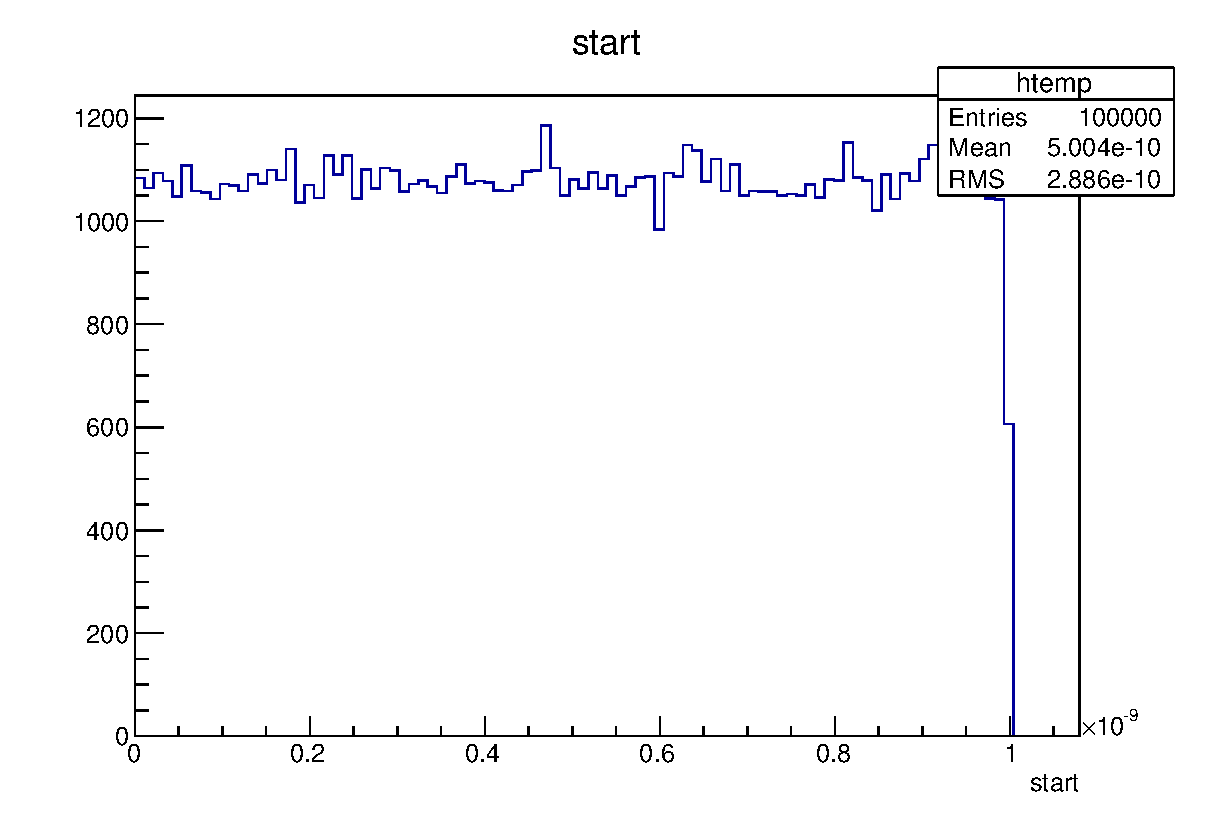
\includegraphics[width = 70mm]{./picture/meettreecanvas1.eps}
  \end{center}
  \caption{\texttt{tree->Draw("start")}実行によって表示される\texttt{start}のヒストグラム}
  \label{Fig:meettreecanvas1}
 \end{minipage}
 \begin{minipage}{0.45\hsize}
  \begin{center}
   \includegraphics[width = 70mm]{./picture/meettreecanvas2.eps}
  \end{center}
  \caption{\texttt{tree->Draw("stop")}実行によって表示される\texttt{stop}のヒストグラム}
  \label{Fig:meettreecanvas2}
 \end{minipage}
\end{figure}


何もしなければbin数やヒストグラムの領域は自動で決まるが設定することももちろん出来る。
\begin{verbatim}
	root [5] tree->Draw("start>>h(100, 0., 1e-9)")
\end{verbatim}
などとすればわかるだろう。

  \subsection{練習}
  \begin{enumerate}
   \item コマンドライン上ででtdcの値格納用のヒストグラムのを用意した後、TDCのヒストグラムを描け。
	 \begin{description}
	  \item[ヒント] \url{http://root.cern.ch/root/html/TTree.html#TTree:Draw@2}
	 \end{description}
   \item tdcをx軸、startをy軸とした図\ref{Fig:meettreecanvas3}のような2次元ヒストグラムをコマンドラインから描け。
	 \begin{figure}[htbp]
	  \begin{center}
	   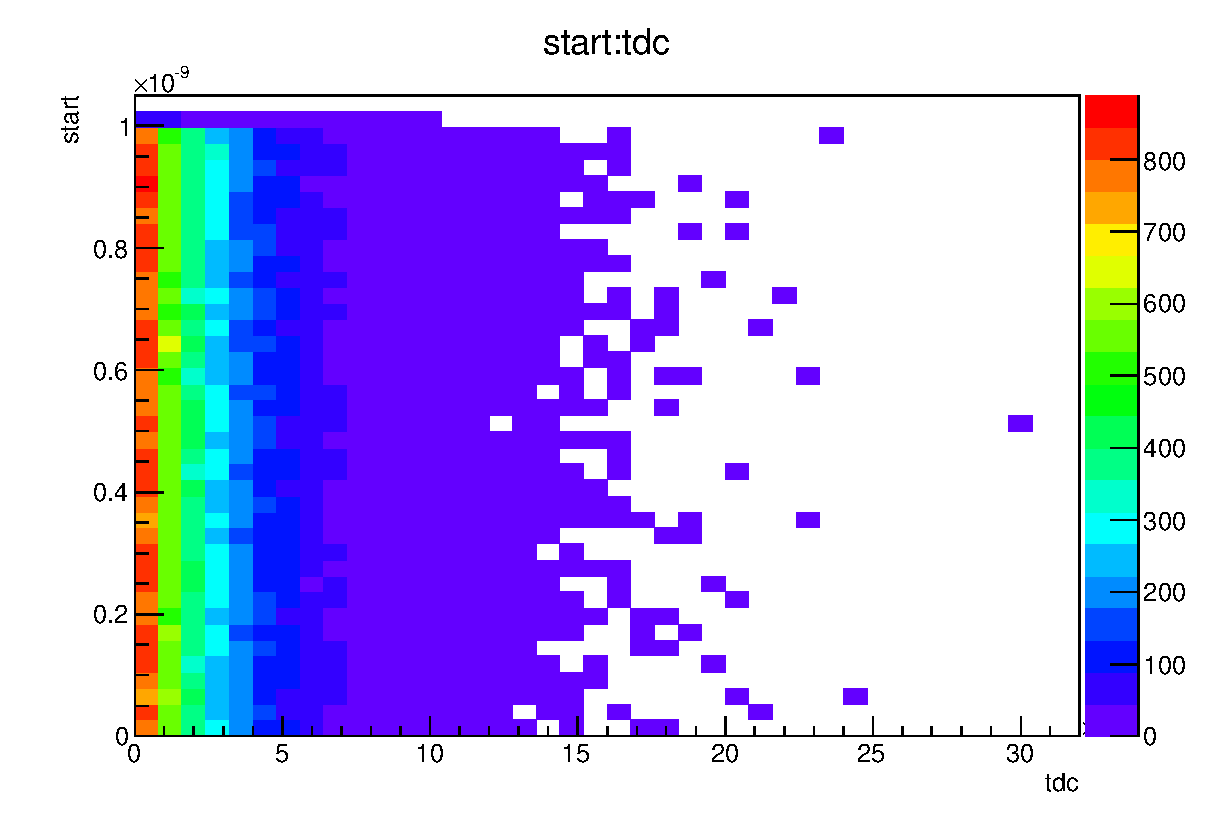
\includegraphics[width = 100mm]{./picture/meettreecanvas3.eps}
	  \end{center}
	  \caption{\texttt{start}実行によって表示される\texttt{start}のヒストグラム}
	  \label{Fig:meettreecanvas3}
	 \end{figure}


	 \begin{description}
	  \item[ヒント] \url{http://root.cern.ch/root/html/THistPainter.html#HP01c}
	 \end{description}
  \end{enumerate}

  \subsection{解答例}
  \begin{enumerate}
   \item コマンドライン上ででtdcの値格納用のヒストグラムのを用意した後、TDCのヒストグラムを描け。
\begin{verbatim}
	root [] TH1D *h = new TH1D("h", "h", 100, 0., 8000e-9)
	root [] tree->Draw("tdc>>h")
	Info in <TCanvas::MakeDefCanvas>:  created default TCanvas with name c1
\end{verbatim}
   \item tdcをx軸、startをy軸とした図\ref{Fig:meettreecanvas3}のような2次元ヒストグラムをコマンドラインから描け。
\begin{verbatim}
	root [] tree->Draw("start:tdc","","colz")
\end{verbatim}
  \end{enumerate}


  %%%%%%%%%%%%%%%%%%%%%%%%%%%%%%%%%%%%%%%%%%%%%%%%%%%%%%%%%%%%%%%%%%%%%%%%%%%%%%%%%
  %%        %%%        %%%        %%%        %%%        %%%         %%%  %%%%  %%%
  %%  %%%%%%%%%  %%%%%%%%%  %%%%%%%%%%%%  %%%%%%%%%  %%%%%%  %%%%%  %%%    %%  %%%
  %%        %%%        %%%  %%%%%%%%%%%%  %%%%%%%%%  %%%%%%  %%%%%  %%%  %  %  %%%
  %%%%%%%%  %%%  %%%%%%%%%  %%%%%%%%%%%%  %%%%%%%%%  %%%%%%  %%%%%  %%%  %%    %%%
  %%        %%%        %%%        %%%%%%  %%%%%%        %%%         %%%  %%%   %%%
  %%%%%%%%%%%%%%%%%%%%%%%%%%%%%%%%%%%%%%%%%%%%%%%%%%%%%%%%%%%%%%%%%%%%%%%%%%%%%%%%%
 \section{Treeから読んで描く}

 \begin{itembox}{\texttt{meettree2.cpp}}
\begin{verbatim}
	#include "TCanvas.h"
	#include "TFile.h"
	#include "TH1D.h"
	#include "TTree.h"

	TH1D *meettree2(char *InputRootFileName){

	TCanvas *c1 = new TCanvas("c1", "c1") ;
	TFile *file = new TFile(InputRootFileName,"READ") ;
	TTree *t = (TTree*)file->Get("tree") ;

	TH1D *h = new TH1D("h","TDC",100, 0., 8000e-9) ; // 8000[ns]
	t->Draw("tdc>>h") ;

	c1->cd() ;
	h->Draw() ;

	return h ;
	}
\end{verbatim}
 \end{itembox}


  \subsection{練習}
  \begin{enumerate}
   \item プログラムの挙動を理解せよ。
	 \begin{description}
	  \item[ヒント] \url{http://root.cern.ch/root/html/TFile.html#TFile:TFile@2}
	  \item[ヒント] \url{http://root.cern.ch/root/html/TDirectoryFile.html#TDirectoryFile:Get}
	 \end{description}
   \item これまでの知識を動員して、\verb|meettree2.cpp|を改良せよ。
	 具体的には軸に単位を追加したり、
	 自動的にFitしたりするなどせよ。
  \end{enumerate}

  \subsection{解答例}
